%----------------------------------------------------------------------------------------
%	MODELLO
%----------------------------------------------------------------------------------------

%\subsection{Il modello}
%\label{sec:modello}
%
%Nella Sezione~\ref{sec:entita_coinvolte} sono state individuate ed analizzate le entità che caratterizzano il sistema. La fase successiva consiste nel definire le interazioni %che legano le suddette entità, in maniera tale da poter derivare un modello per il sistema.

\subsubsection{Interazione tra giocatori: il controllore}
\label{sec:modello_interazione_giocatori}

%Interazione tra giocatori: il controllore.
I giocatori sono i principali attori del sistema. Un giocatore si sposta dentro e fuori dal campo, è in grado di compiere diversi tipi di azioni (Sezione~\ref{sec:analisi_giocatori}), che decide sia sulla base del proprio stato che dello stato della propria squadra e della partita. Un aspetto fondamentale vede i giocatori, così come avviene nel mondo reale, operare in maniera parallela e concorrente tra di loro: questo implica che i risultati delle loro azioni debbano riflettersi sullo stato di gioco, che come descritto in Sezione~\ref{sec:entita_coinvolte_stato}, detiene tutte le informazioni che definiscono la partita in un dato istante. Si pone però un problema: i giocatori, per poter conoscere le informazioni che permetteranno loro di decidere la prossima azione da compiere, i giocatori devono accedere allo stato, che tuttavia è unico. E' dunque necessario regolamentare l'accesso a tale risorsa, in maniera tale da preservarne la consistenza e la correttezza.\\

L'organo che si occupa di permettere l'interazione tra diversi giocatori è il \textit{controllore}. In quanto entità centrale di controllo, i suoi molteplici compiti possono essere raggruppati come segue:

\begin{enumerate}
	\item Permettere ai giocatori di accedere allo stato, sia per leggerne le informazioni sia per poterle modificare
	\item Sequenzializzare gli accessi allo stato da parte dei giocatori, al fine di non creare inconsistenze sulle informazioni in esso contenute
	\item Ricoprire il ruolo di arbitro di gioco ``onnisciente'' (verrà dettagliato in Sezione~\ref{sec:modello_verifica_arbitro})
\end{enumerate}

Come già accennato precedentemente, un giocatore decide la sua prossima mossa sulla base dello stato corrente della partita: ad esempio, trovandosi in possesso della palla nell'area avversaria e senza nessun giocatore a marcarlo, è ragionevole che il giocatore decida di tirare per provare a realizzare un goal. Al tempo stesso, l'azione che egli compie si ripercuote sullo stato della partita, andandone a modificare una parte: di nuovo, se il giocatore segna, il punteggio della partita cambia e i giocatori ritornano in posizione di partenza per ricominciare il gioco. Questo meccanismo mette in luce una necessità tale per cui le operazioni che alterano lo stato siano quanto più possibile sequenziali ed atomiche. Sebbene questo argomento verrà trattato ampiamente nel Capitolo~\ref{sec:analisi_architetturale}, è importante capire il motivo dell'importanza di queste due caratteristiche.\\

L'assunzione di atomicità si rivela particolamente critica quando si assume di operare in condizioni di prerilascio dei processi. Sotto questa condizione, un processo correntemente in esecuzione può essere ``temporaneamente fermato'' (prerilasciato) in favore di un altro processo, che entra quindi in esecuzione al suo posto; una simile condizione si verifica, ad esempio, se il processo corrente ha una priorità inferiore di quello che vuole subentrare. Per spiegare come il prerilascio minacci la consistenza dello stato della partita, si consideri una situazione dove due giocatori avversari si contendono il possesso della palla, che giace inerte in mezzo a loro. Entrambi i giocatori leggono lo stato e avviano il processo di decisione della prossima azione. Tuttavia, il processo relativo al primo giocatore viene prerilasciato. Nel frattempo, il secondo giocatore conquista la palla e si muove verso la porta avversaria. Quando il primo giocatore torna in esecuzione si trova in uno stato inconsistente, in quanto lo stato è cambiato senza che lui lo sappia. Ancora peggio, se il primo giocatore procede con la scrittura della sua azione, lo stato verrà modificato erroneamente, potenzialmente togliendo il possesso di palla al secondo giocatore.\\

Arrivati a questo punto, serve quindi definire come i giocatori vanno effettivamente a modificare lo stato di gioco. Il modello prevede che sia solamente il controllore ad effetuare le scritture vere e proprie sulla base delle azioni decise e sottoposte da parte dei giocatori. Tali richieste vengono valutate in modo sequenziale, andando così a modificare lo stato con una azione alla volta evitando così condizioni di inconsistenza sullo stato.\\

Come detto in precedenza, all'inizio di ogni suo turno un giocatore deve prendere coscienza di quale sia lo stato attuale di gioco, decidere la prossima mossa sulla base di quest'ultimo e sottoporla al controllore per modificare lo stato. Questo meccanismo, abbinato al fatto che i giocatore eseguono in modo potenzialmente parallelo e che ogni richiesta viene elaborata in maniera sequenziale, farebbe pensare ad una soluzione che prevede un accesso esclusivo al controllore da parte di un giocatore per tutta la durata del suo ciclo di esecuzione. L'idea alla base della soluzione è quindi quella di scomporre la routine del turno come segue:\\

\begin{enumerate}
	\item il giocatore richiede al controllore lo stato di gioco
	\item viene effettuata una fase di computazione con la quale decide la prossima mossa
	\item richiede al controllore di applicare l'azione scelta allo stato.
\end{enumerate}

Si ha quindi che la fase di lettura e la fase di scrittura (primo e terzo punto) vengono effettuate “online”, ovvero tramite accesso esclusivo al controllore; la parte di scelta della prossima azione avviene invece “offline”, quindi senza la necessità di interagire con esso. In questo modo si guadagna un parallelismo potenziale nella seconda fase, permettendo così ai giocatori di non interferire tra di loro nella decisione della prossima mossa.

\subsubsection{Verifica sullo stato di gioco: l'arbitro}
\label{sec:modello_verifica_arbitro}

Affiché una partita si svolga secondo le regole e le modalità stabilite dal gioco del calcio c'è bisogno di un arbitro che regoli l'andamento del gioco. Le mansioni dell'arbitro sono molteplici:

\begin{itemize}
	\item Sancire l'inizio e la fine dei tempi di gioco (inizio primo tempo - fine primo tempo - inizio secondo tempo - fine partita)
	\item Fermare il gioco e farlo riprendere a seguito (e.g. una rimessa laterale)
	\item Segnalare eventuali irregolarità da parte dei giocatori (e.g. un fallo)
	\item Tenere il conto dei gol segnati da entrambe le squadre, così da decretare il vincitore alla fine della partita
	\item Gestire le richieste di sostituzione e di cambio di formazione da parte degli allenatori
\end{itemize}

L'arbitro deve quindi essere in grado di controllare tutte le mosse dei giocatori, così come lo stato e la posizione della palla e la durata della partita fino a quel momento. Nella realtà, il ruolo dell'arbitro è assegnato ad un essere umano, che quindi non è infallibile: si pensi ad esempio ad un fallo che viene commesso irregolarmente alle sue spalle mentre lui è impegnato ad assegnare un calcio d'angolo. In questa simulazione si assume più semplicemente che l'arbitro sia ``onnisciente'', ovvero abbia la facoltà di analizzare ogni singola mossa di ciascun giocatore e della palla, in maniera da poter segnalare immediatamente ogni irregolarità oppure fermare il gioco all'occorrenza.\\

Si ha così che il controllore, descritto nel paragrafo precedente, ricopre anche il ruolo di arbitro. Questa decisione ha delle ripercussioni non solo nello svolgersi del gioco (l'arbitro è onnisciente), ma anche nell'assegnazione delle risorse di calcolo. Infatti, se l'arbitro fosse soggetto agli stessi vincoli di esecuzione dei giocatori, andrebbe a concorrere assieme a loro per l'esecuzione sulla CPU come task a se stante; questa situazione non si verifica invece nel caso in cui sia il controllore ad essere anche arbitro, essendo l'entità centrale che si occupa di eseguire a tutti gli effetti le mosse dei giocatori. Maggiori dettagli sull'implementazione dell'arbitro verranno esposti in Sezione~\ref{sec:implemetazione_concorrenza}.\\

L'elenco delle funzioni che l'arbitro deve espletare nasconde tuttavia un punto critico su cui è opportuno soffermarsi. I primi quattro punti sono strettamente legati alla componente concorrente della simulazione, ovvero quella che vede l'interazione dei giocatori con il controllore e, in alcuni casi, l'agente di movimento. L'ultimo punto fa invece riferimento alla componente distribuita della simulazione, ovvero quella che si occupa di ricevere e gestire i comandi impartiti dagli allenatori ed eventualmente dalla finestra principale di controllo (che, come verrà esposto successivamente, coincide con la componente che mostra il campo di gioco e lo svolgersi della partita). La differenza sostanziale tra queste due tipologie di eventi è racchiusa nel fatto che gli eventi provenienti dalla componente distribuita non sono deterministici e non seguono nessuna regola di generazione, a differenza degli eventi relativi alla parte concorrente.
La presenza di due sorgenti di eventi introduce un problema significativo, ovvero l'ordine in cui l'arbitro deve processare/consumare quegli eventi. Ad esempio, si consideri una situazione dove si ha una richiesta di sostituzione per il giocatore 1 in favore del giocatore 3 e, allo stesso tempo, sia stato commesso un fallo commesso dal giocatore 1 sul giocatore 2. L'ordine in cui vengono processati questi eventi determina lo stato successivo, che diverge a seconda che si consideri prima uno oppure prima l'altro. Bisogna tenere conto, ad ogni modo, che gli eventi che vengono generati dalla componente distribuita hanno come precondizione il gioco fermo: quindi c'è una stretta dipendenza unidirezionale tra un evento singolo della componente concorrente e gli eventi della componente distribuita. L'approccio da seguire per garantire il massimo livello di correttezza temporale è quindi il seguente: l'arbitro dovrà prima processare l'evento singolo della componente concorrente (che può causare il gioco fermo, nel caso non lo fosse già) e solo poi processare gli eventi della componente distribuita, se le condizioni sono opportune.

\subsubsection{La palla in movimento: l'entità e l'agente di movimento}
\label{sec:modello_palla_agente_movimento}

%La palla in movimento: l'entità e l'agente di movimento.

La palla è una parte fondamentale del modello della simulazione, in quanto il suo possesso viene conteso dai giocatori che devono tirarla in porta, segnando un gol per la loro squadra. Il suo comportamento può essere definito come una macchina a stati, schematizzato nel seguente diagramma:

\begin{figure}[htp!]
	\centering
	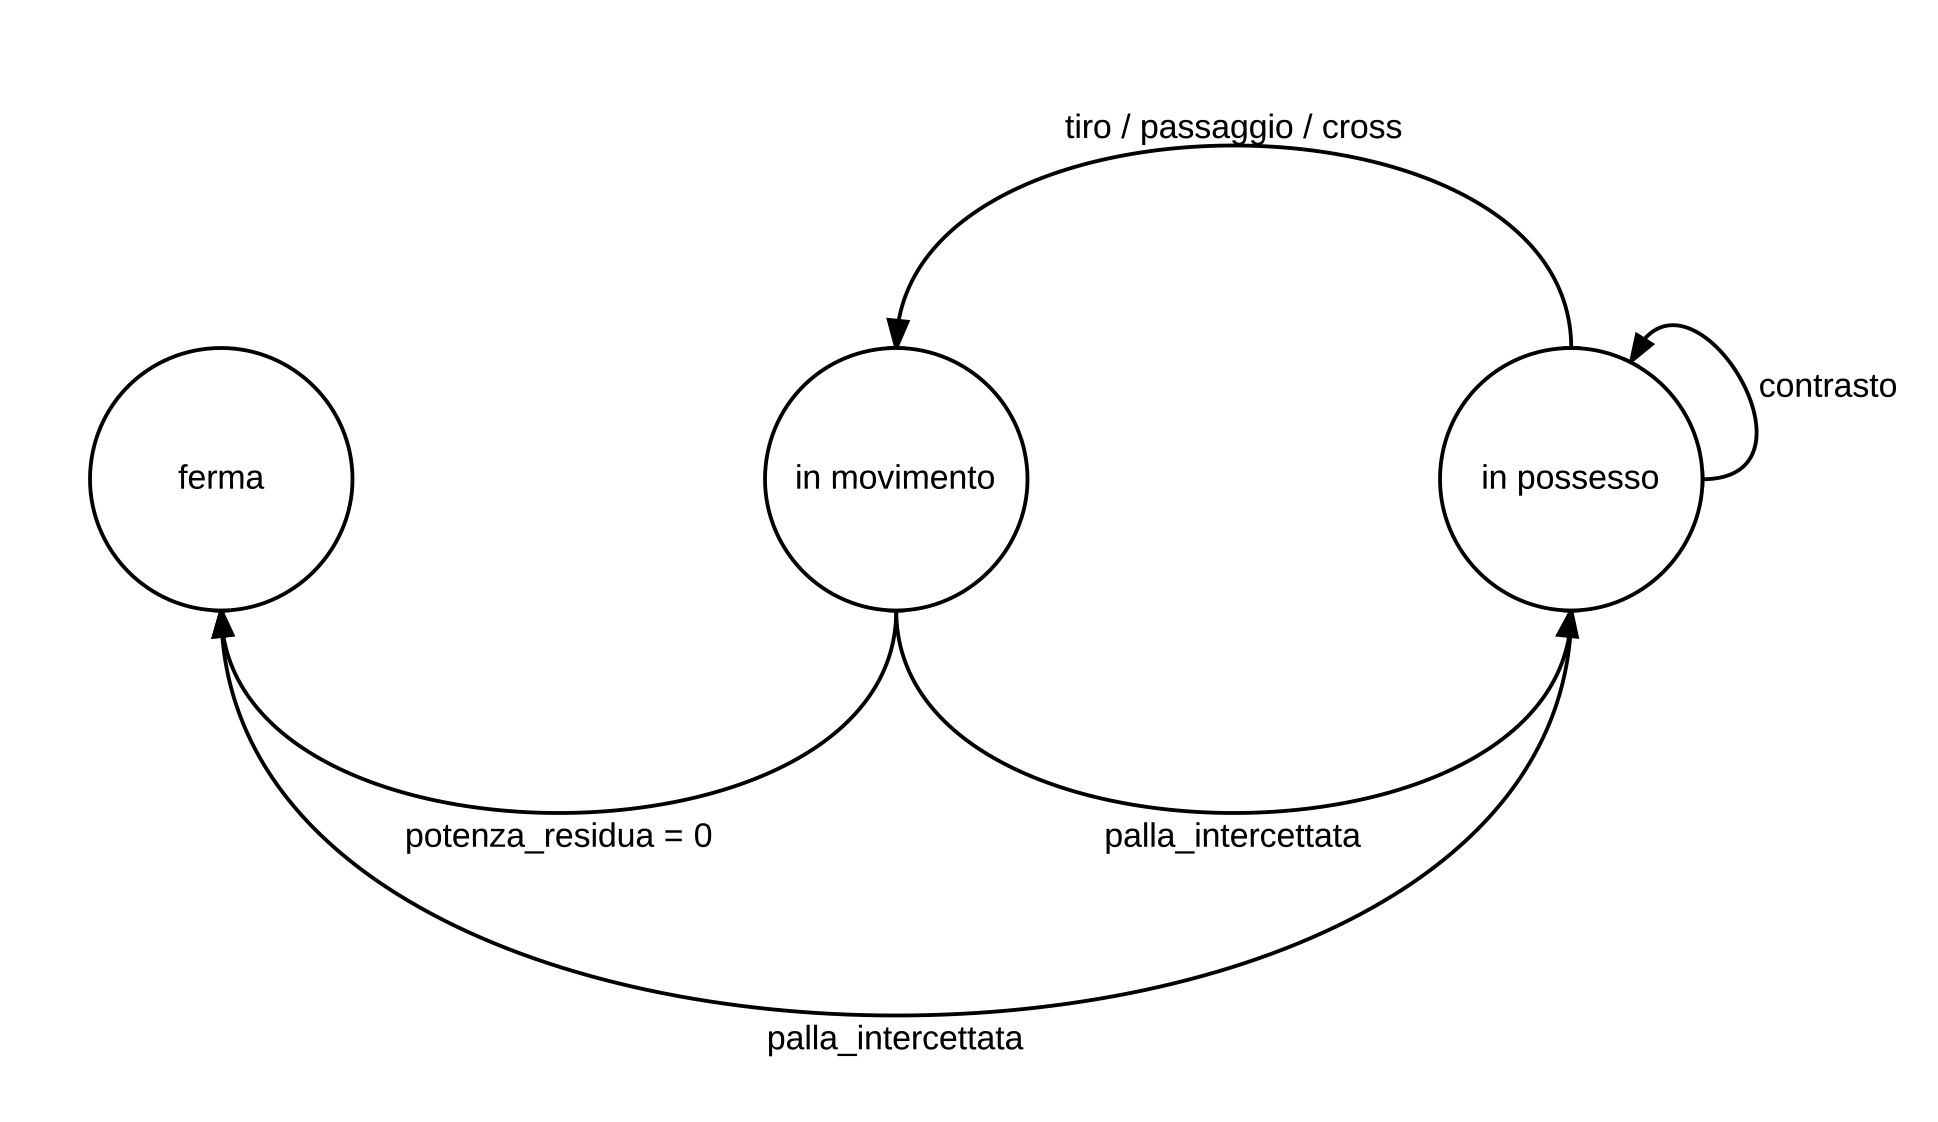
\includegraphics[scale=.8]{images/ball_state_diagram}
\end{figure}

In ogni momento della partita, la palla occupa una delle celle del campo. Nel caso sia posseduta da un giocatore, essi condividono la stessa cella; in caso contrario, la palla occupa la cella in cui si trova. Inoltre, la palla può trovarsi solamente in due stati: quiete e moto. Una palla in movimento si può avere quando il giocatore che la controlla si sposta con essa; inoltre, si ha una palla in movimento anche quando un giocatore la passa verso un altro giocatore oppure effettua un tiro verso la porta avversaria. Al contrario, una palla è inerte se non è controllata da nessun giocatore, solitamente quando un passaggio o un tiro mancano il bersaglio (e.g. un passaggio troppo debole). La palla è quindi una risorsa protetta, che non compie azioni proprie ma che subisce azioni di altre entità attive (i giocatori) e salva di volta in volta la sua posizione aggiornata.\\

Di conseguenza, quando un giocatore effettua un passaggio oppure un tiro, la palla deve essere spostata da un'entità che però non può essere il giocatore stesso: in altre parole, si tratta di simulare l'impressione di un moto alla palla a seguito di un'azione del giocatore che la controlla. Questa mansione è ricoperta dal cosiddetto \textit{agente di movimento}. L'agente di movimento è un'entità reattiva concorrente agli altri giocatori, il cui unico compito è quello di spostare la palla in una determinata direzione fino a che la potenza ad essa impressa è sufficiente a farla avanzare alla cella successiva. Una volta completato il suo compito, smette di eseguire in attesa del prossimo spostamento da effettuare. In alcuni casi, l'agente di movimento viene volutamente bloccato attraverso l'arbitro, ad esempio nel caso in cui la palla esca dal campo e sia necessario assegnare una rimessa oppure un calcio d'angolo.

\subsubsection{Modifiche sulle squadre: gli allenatori}
\label{sec:modello_squadre_allenatori}

%Modifiche sulle squadre: gli allenatori.

Nel gioco del calcio i giocatori di ciascuna squadra vengono coordinati dal proprio allenatore, che ha il compito di scegliere come disporre i giocatori in campo (la formazione) e di effettuare delle sostituzioni, come conseguenza di un infortunio o più semplicemente per una scelta tattica. In questa simulazione i due allenatori rappresentano due componenti distribuite separate, che comunicano con l'unità centrale di controllo. Ciascun allenatore ha la facoltà di prendere le seguenti decisioni:

\begin{itemize}
	\item effettuare un cambio di formazione per la propria squadra
	\item effettuare una sostituzione di un giocatore con un suo compagno presente in panchina
\end{itemize}

Le decisioni prese da un allenatore hanno come precondizione necessaria il gioco fermo: sarà pertanto l'arbitro a dover esaminare e successivamente accettare le richieste di un allenatore solo quando le condizioni lo permettono. Nel caso di un semplice cambio di formazione, la decisione dell'allenatore viene applicata sulla squadra, cosicché i giocatori al proprio turno successivo sappiano che la loro posizione di riferimento è cambiata. Diverso e più complesso è invece il caso della sostituzione. La sequenza di operazioni che seguono una richiesta di sostituzione si possono schematizzare come segue:

\begin{enumerate}
	\item L'arbitro riceve la richiesta di sostituzione e, non appena il gioco è fermo, procede a notificarlo ai giocatori
	\item Ciascun giocatore, prima di decidere la propria mossa, controlla se l'allenatore ha deciso di sostituirlo con un compagno
	\item Nel caso del giocatore interessato alla sostituzione, esso si dirige verso la panchina (eventualmente lasciando la palla dove si trova)
	\item Una volta giunto in panchina, il suo compagno prende il suo posto in campo e si dirige verso la propria posizione di riferimento
	\item L'arbitro, ad ogni turno, controlla se il giocatore entrante ha raggiunto la posizione di riferimento e, in quel caso, sancisce la ripresa del gioco
\end{enumerate}

Il comportamento sopra descritto vale anche nel caso di più sostituzioni simultanee, che vedono i giocatori uscire ed entrare nel campo allo stesso tempo.\\

Ciascun allenatore ha inoltre una visione meno precisa del gioco e riceve pertanto un sottoinsieme degli eventi che caratterizzano una partita: dal punto di vista decisionale è infatti poco interessante per un allenatore conoscere ogni singolo movimento di ogni giocatore. Si ha quindi che l'allenatore viene notificato solo in caso di eventi ``salienti'', che come descritto nel Capitolo~\ref{sec:analisi_architetturale}, sono stati denominati \textit{Game Events}.

%\subsubsection{Gestione delle fasi di gioco: entità di gioco}
%\label{sec:modello_fasi_game_entity}
%
%%Gestione delle fasi di gioco: entità di gioco.
%
%[secondo me non va messa qui, è prettamente implementativa]
